\section{Rango din\'amico}
Se calcul\'o la transferencia desde la entrada hasta la salida de cada celda. Se buscaron los puntos de transferencia m\'axima y m\'inima dentro del rango de la banda pasante, obtenidos mirando la figura \ref{fig:DR}. Luego, con estos puntos se obtuvo el rango de amplitudes de la se\~nal de entrada para los cuales la se\~nal no cae por debajo del piso de ruido (considerado 50mV) ni supera la salida m\'axima del op-amp (10V, valor m\'inimo especificado en la hoja de datos) usando la ecuaci\'on \ref{eq:DR}. 

\begin{figure}[H]
	\centering
	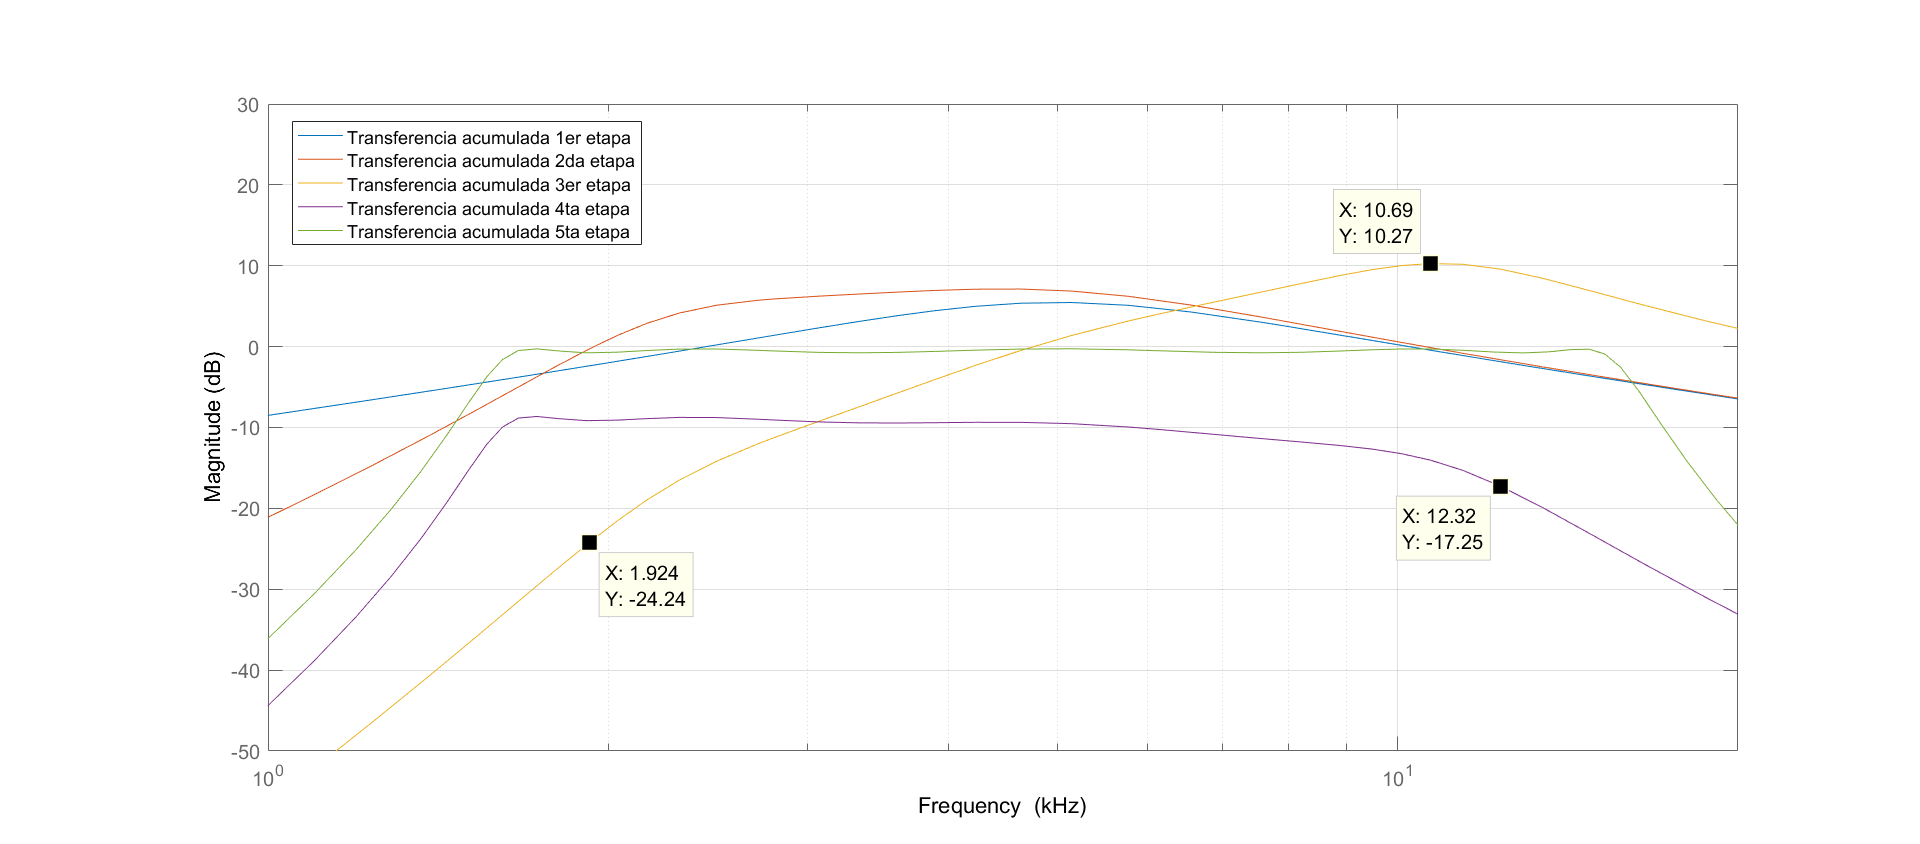
\includegraphics[width=\textwidth]{imagenes/DR.png}
	\caption{Transferencias entre la salida de cada etapa y la entrada al circuito}
	\label{fig:DR}
\end{figure}

\begin{equation}
	H=20\, log\left(\frac{V_o}{V_i}\right) \\
	\Rightarrow V_i = 10^{-\frac{H}{20}}\cdot V_o
	\label{eq:DR}
\end{equation}

\begin{table}
	\centering
	\begin{tabular}{||ccc||}
	\hline 
	 & Transferencia & Tensi\'on de entrada \\ 
	\hline 
	M\'inimo & -24.24 dB (salida 3er etapa, 1.92KHz) & 0.16V \\ 
	\hline 
	M\'aximo & 10.27 dB (salida 3er etapa, 10.27KHz) & 3.1V \\ 
	\hline 
	\end{tabular} 
	\caption{Rango din\'amico para la banda pasante}
	\label{tab:DR}
\end{table}


Para poder observar una atenuaci\'on de 45 dB en la banda atenuada, de la ecuaci\'on \ref{eq:DR} se obtiene que se necesita una tensi\'on de entrada de 1.7V.
